\documentclass[tikz,border=8pt]{standalone}
\usepackage{tikz}
\usepackage{amsmath, amssymb}

\usetikzlibrary{shapes.geometric, positioning}

\begin{document}

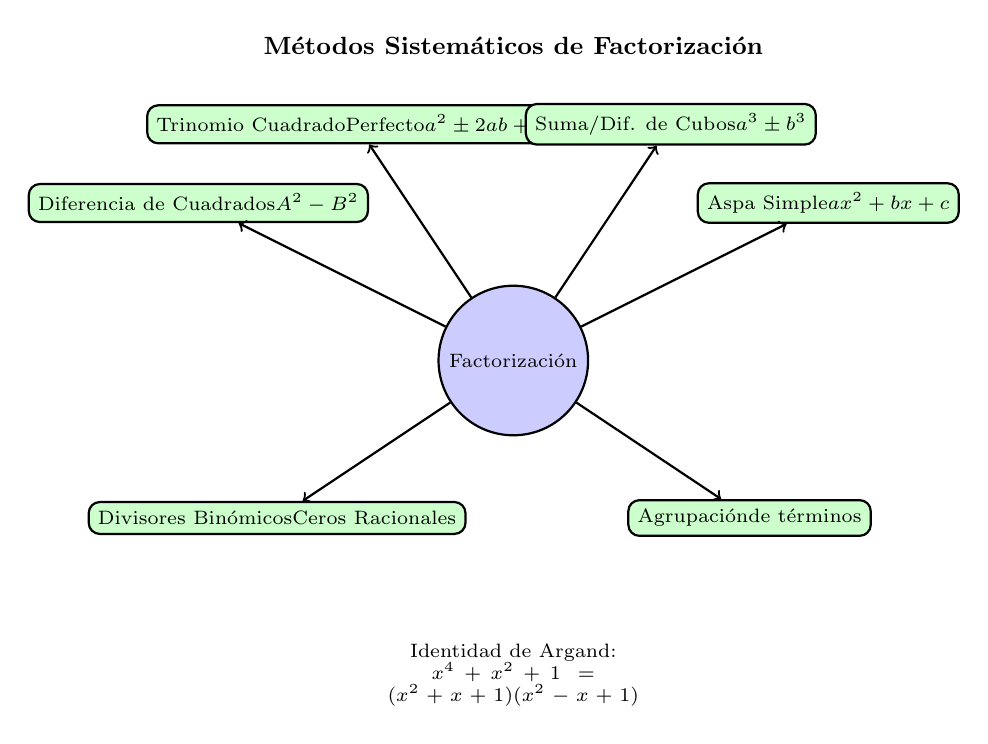
\begin{tikzpicture}[scale=1.0]

  % Nodo central
  \node[draw, thick, circle, fill=blue!20, font=\scriptsize] (centro) at (0, 0) {Factorización};

  % Nodos alrededor
  \node[draw, thick, rectangle, rounded corners, fill=green!20, font=\scriptsize] (dif_cuad) at (-4, 2) {Diferencia de Cuadrados\\$A^2 - B^2$};
  \node[draw, thick, rectangle, rounded corners, fill=green!20, font=\scriptsize] (tcp) at (-2, 3) {Trinomio Cuadrado\\Perfecto\\$a^2 \pm 2ab + b^2$};
  \node[draw, thick, rectangle, rounded corners, fill=green!20, font=\scriptsize] (cubos) at (2, 3) {Suma/Dif. de Cubos\\$a^3 \pm b^3$};
  \node[draw, thick, rectangle, rounded corners, fill=green!20, font=\scriptsize] (aspa) at (4, 2) {Aspa Simple\\$ax^2 + bx + c$};
  \node[draw, thick, rectangle, rounded corners, fill=green!20, font=\scriptsize] (grupo) at (3, -2) {Agrupación\\de términos};
  \node[draw, thick, rectangle, rounded corners, fill=green!20, font=\scriptsize] (gauss) at (-3, -2) {Divisores Binómicos\\Ceros Racionales};

  % Conexiones
  \draw[->, thick] (centro) -- (dif_cuad);
  \draw[->, thick] (centro) -- (tcp);
  \draw[->, thick] (centro) -- (cubos);
  \draw[->, thick] (centro) -- (aspa);
  \draw[->, thick] (centro) -- (grupo);
  \draw[->, thick] (centro) -- (gauss);

  % Título
  \node[font=\small\bfseries] at (0, 4) {Métodos Sistemáticos de Factorización};

  % Identidad de Argand
  \node[align=center, text width=4cm, font=\scriptsize] at (0, -4) {
    Identidad de Argand:\\
    $x^4 + x^2 + 1 = (x^2+x+1)(x^2-x+1)$
  };

\end{tikzpicture}

\end{document}
